\setcounter{ExampleCounter}{1}
\begin{center}

\includegraphics[width=0.8\textwidth]{Millionaire}\\
\text{} \hfill {\small\color{gray}Image by Wikipedia user Idea SV is licensed under CC BY-SA 3.0}
\end{center}

Who wants to be a millionaire?  More realistically, who \emph{doesn't} want to be a millionaire?  It may sound like an unattainable goal, but in this section, you'll learn how you can join the millionaire club by taking advantage of the power of compound interest.

If you forget everything else you learn here, don't forget this one lesson:
\begin{center}
{\LARGE START SAVING EARLY}
\end{center}

The results speak for themselves:
\begin{center}
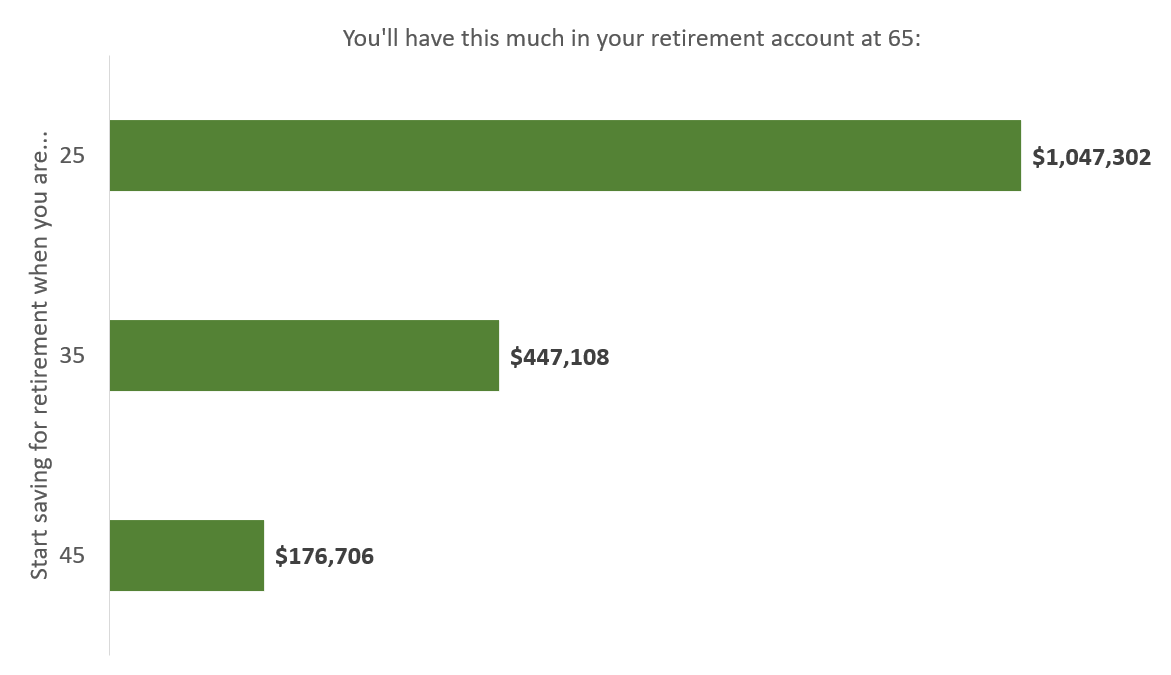
\includegraphics[width=0.8\textwidth]{RetirementGoals}
\end{center}

This graph shows how much you can accumulate if you can save \$300 a month, assuming that you receive an 8\% annual return on your investments, a fairly typical result if, for instance, you invest in index funds, which are mutual funds designed to track the market as a whole over the long term.

That may sound like a lot to save, but this is about the amount that many people spend on a car payment.  What this means is that with relatively small sacrifices, such as driving used cars instead of new ones, you can someday see your retirement account cross the \$1,000,000 threshold.

Let's dig into that chart a bit more.  Notice that if you wait until age 35 to start saving, you won't just save a \emph{bit} less than you would if you started saving earlier; you'll wind up with \emph{less than half}, just by waiting 10 years.  Maybe you can't afford to save \$300 a month right now, but if you can afford \$100 a month, start there!

Why is there such a dramatic difference?  It's all due to compound interest, and we learned in the last section that compound interest really flexes its muscles when you give it plenty of time.  Those 10 years between ages 25 and 35 are the most important years in the process, because they are the first years, and the money saved then has the most time to grow.

To show this, let's break down the amount that you will actually deposit in each case, versus the amount you'll earn in interest:
\begin{center}
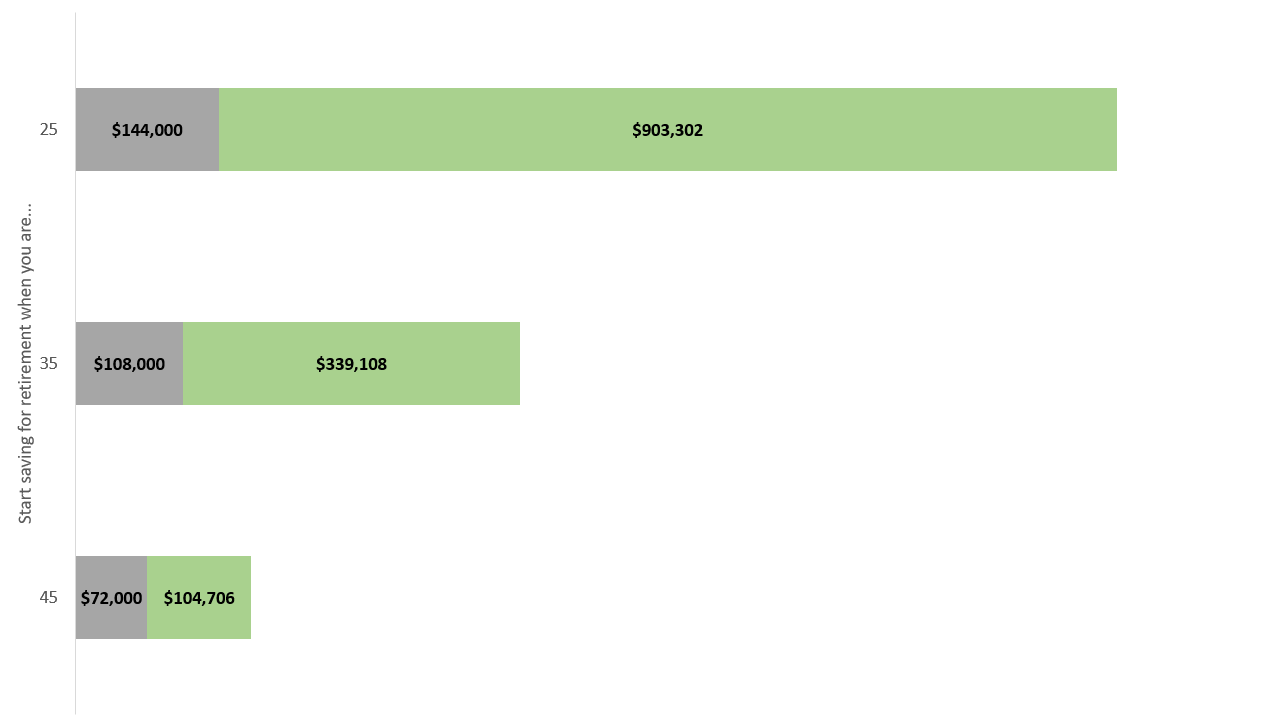
\includegraphics[width=0.8\textwidth]{RetirementGoalsWithInterest}
\end{center}

Notice that if you wait until age 45 to start saving, you'll end up depositing half of what you would if you started at 25, but your final balance will be about \emph{one sixth} of what it could be.  Another way to look at it is that starting at age 25 multiplies your money by over seven times (the ratio of what you actually save and what interest adds), but starting at age 45 only multiplies your money by about two and a half.

In this section, you'll learn how all of those values were calculated, but the conclusion should already be clear: don't wait any longer to start saving!

\subsection{Annuities}
The term \emph{annuity} simply refers to a series of recurring payments.  This is different from what we did in the last section, where we assumed that a single lump-sum deposit was made and a single withdrawal was made later.  We haven't yet dealt with accounts that take regular deposits, but that's what you do for any kind of long-term savings plan: use small, regular payments to grow over time.

In this section, we'll discuss two types of annuities, which are similar, but the formulas are slightly different.

\begin{formula}{Types of Annuity}
\paragraph{Savings Annuity} This is the kind that you use to save for retirement; you make regular deposits over time, and the balance slowly grows because of two factors: your deposits and the accruing interest.

\paragraph{Payout Annuity} When you retire, you stop making payments into your retirement plan, and you start receiving regular payouts instead, which replace your paycheck.  In this case, we start the problem with a lump sum (what you managed to save) and compare that lump sum with the payment amount that you receive.
\end{formula}

If you do more research on annuities, you'll find that there are other variations, such as lifetime annuities, or that annuities apply in other situations (usually some large payment such as life insurance or lottery winnings can be paid out using annuities), but our focus will be on retirement savings, since that's the most common scenario.

For our purposes, the basic process looks something like this: starting today, you can deposit money into a savings annuity, and we can calculate what your final balance will be when you retire.  Then, we can fast-forward to the day of retirement, and projecting how much your account will hold, we can find out how much you can expect to receive as a monthly payment in retirement.  We can also work backward from how much you'll need in retirement to calculate the balance you need when you retire, then work backward again to calculate how much you'll need to start saving.
\vfill
\pagebreak

\subsection{Savings Annuities}

Let's start with a simple example to illustrate how a savings annuity works.

\begin{example}[https://www.youtube.com/watch?v=KOIRAWGh9vM&list=PLfmpjsIzhztsZtnb7HnXrQ8SLoiOCIcAM&index=25]{Savings Annuity}
Suppose you deposit \$100 into a savings account at the end of each year.  If you earn 5\% interest compounded annually, how much will the account hold at the end of 3 years?  How much interest did the account earn?\\

\marginnote{\bfseries Solution}
At the end of the first year, the account holds the \$100 that you deposit then:
\[F_1 = \$100\]
The second year, this \$100 earns interest, plus you deposit another \$100 at the end of the year:
\[F_2 = \$100(1+0.05) + \$100 = \$205\]
The third year, this \$205 earns interest, plus you deposit another \$100 at the end of the year:
\[F_3 = \$205(1+0.05) + \$100 = \$315.25\]
We could continue this pattern indefinitely, but each year, we only need to use the simple interest formula to see how much the previous year's balance has grown, and then add in that year's deposit.\\

At the end of the three years, the account holds \$315.25, and since we deposited a total of \$300 (\$100 each year for 3 years), the account earned a total of \$15.25 in interest.
\end{example}

In theory, we could do that every time we need to calculate the value of an annuity, but that would get tedious very quickly.  The following formula is derived based on that process (details are at the end of this section, in case you'd like to see the algebra).

\begin{formula}{The Future Value of a Savings Annuity}
If regular deposits of $PMT$ are made $n$ times per year into an annuity paying an interest rate of $r$ compounded $n$ times per year, the future value of the annuity at the end of $t$ years is given by
\[F=\dfrac{PMT\left[\left(1+\dfrac{r}{n}\right)^{nt}-1\right]}{\left(\dfrac{r}{n}\right)}\]
\end{formula}

This formula looks complicated, but with a little practice, you'll be able to use it, for instance, to verify the numbers in the retirement discussion at the beginning of the section.

By the way, we may also start by determining how much we want the account to hold at the end, and use that to calculate $PMT$.  To do that, we need to solve the formula above for $PMT$, which means multiplying both sides by $r/n$ and dividing both sides by the expression in brackets:
\[PMT = \dfrac{F\left(\dfrac{r}{n}\right)}{\left(1+\dfrac{r}{n}\right)^{nt}-1}\]
You can choose to keep this formula handy as well, or you can simply do the algebra each time.  It helps to enter all the values and simplify as much as possible on the right hand side, and then simply divide $F$ by that simplified value.
\pagebreak

\begin{example}[https://www.youtube.com/watch?v=X1oXL3ZjcCU&list=PLfmpjsIzhztsZtnb7HnXrQ8SLoiOCIcAM&index=26]{Traditional IRA}
A traditional individual retirement account (IRA) is a retirement account in which the money you invest is tax-exempt (you can deduct your contributions on your income tax return) until you withdraw it.  Thus, taxes are deferred until you retire.  If you deposit \$250 each month into an IRA earning 7\% interest, how much will you have in the account after 35 years?

\sol
Organize the given information:
\begin{center}
\begin{tabular}{r l l}
$PMT$ & \$250 & The regular deposit\\
$r$ & 0.07 & 7\% annual rate\\
$n$ & 12 & Deposits are made monthly\\
$t$ & 35 & Deposits are made for 35 years
\end{tabular}
\end{center}

Putting it all together in the formula:
\begin{align*}
F &= \dfrac{\$250\left[\left(1+\dfrac{0.07}{12}\right)^{(12)(35)}-1\right]}{\left(\dfrac{0.07}{12}\right)} = \boxed{\$450,264}
\end{align*}

Notice\marginnote{$(\$250)(12)(35) = \$105,000$} that you deposited \$250 every month, 12 months a year for 35 years, for a total of \$105,000.  That means that the account earned approximately $\$450,264-\$105,000 = \$345,264$ in interest, or to put it another way, the deposits more than quadrupled due to interest.
\end{example}

%\paragraph{Note:} we rounded here to the nearest dollar, since the dollar amount is so large, making the cents less significant.  There's no rule about this, but simply a matter of preference.

\begin{try}[http://hartleymath.com/versatilemath/tryit/\#/financial-mathematics--future-value-for-savings-annuity]
If you deposit \$800 every year into a traditional IRA earning 4\% interest, how much will the account hold after 25 years?
\end{try}

There is another common type of retirement account: the Roth IRA.  The idea behind a Roth IRA was originally proposed in 1989 by Senator William Roth of Delaware and established by the Taxpayer Relief Act of 1997.

The differences between traditional and Roth IRAs do not affect the calculations in the examples, but you may hear both terms discussed, so we'll include a short comparison here just for your interest (you can skip this if you prefer).

\checkoddpage
\ifoddpage{
\begin{adjustwidth}{-0.25in}{-1.75in}
\begin{proc}{Traditional vs. Roth IRA}
The main difference between the two types of IRA (individual retirement accounts) revolves around taxes.  With a traditional IRA, contributions are tax-free (you can deduct these on your tax return) and you pay taxes when you withdraw the funds in retirement.  Roth IRA contributions, on the other hand, are taxed when you make them, but when you make withdrawals after retiring, you won't pay taxes then.\\

Thus, when comparing the two, the question is: do you expect to pay higher taxes now, or when you are retired?  It's hard to know for sure, because your income may be higher or lower than it is now, and many of the deductions you'll take advantage of in the near term (like mortgage insurance, dependent expenses, or education costs) will not apply when you are retired.\\

There are other qualitative differences, like the fact that a traditional IRA will require you to start withdrawing when you reach 70.5 years of age; Roth IRAs don't have that restriction, making them a popular vessel for transferring wealth to inheritors.

\paragraph{Contribution Limits (2020)}
The most you can contribute to either kind of IRA (or a combination of the two) in a single year is \$6,000 if you're younger than 50, or \$7,000 if you're 50 or older.

\paragraph{Income Limits (2020)}
Traditional IRAs have no income limits, but you can't contribute to Roth IRAs if you make too much money.  For instance, the current limit for single individuals is \$124,000, and \$196,000 for married couples; if your adjusted income is higher, you can only contribute to a traditional IRA that year.\\

One final note: both kinds of IRA allow first-time homebuyers to withdraw up to \$10,000 to pay for qualified housing costs.
\end{proc}
\end{adjustwidth}
} \else{
\begin{adjustwidth}{-1.75in}{-0.25in}
\begin{proc}
The main difference between the two types of IRA (individual retirement accounts) revolves around taxes.  With a traditional IRA, contributions are tax-free (you can deduct these on your tax return) and you pay taxes when you withdraw the funds in retirement.  Roth IRA contributions, on the other hand, are taxed when you make them, but when you make withdrawals after retiring, you won't pay taxes then.\\

Thus, when comparing the two, the question is: do you expect to pay higher taxes now, or when you are retired?  It's hard to know for sure, because your income may be higher or lower than it is now, and many of the deductions you'll take advantage of in the near term (like mortgage insurance, dependent expenses, or education costs) will not apply when you are retired.\\

There are other qualitative differences, like the fact that a traditional IRA will require you to start withdrawing when you reach 70.5 years of age; Roth IRAs don't have that restriction, making them a popular vessel for transferring wealth to inheritors.

\paragraph{Contribution Limits (2020)}
The most you can contribute to either kind of IRA (or a combination of the two) in a single year is \$6,000 if you're younger than 50, or \$7,000 if you're 50 or older.

\paragraph{Income Limits (2020)}
Traditional IRAs have no income limits, but you can't contribute to Roth IRAs if you make too much money.  For instance, the current limit for single individuals is \$124,000, and \$196,000 for married couples; if your adjusted income is higher, you can only contribute to a traditional IRA that year.\\

One final note: both kinds of IRA allow first-time homebuyers to withdraw up to \$10,000 to pay for qualified housing costs.
\end{proc}
\end{adjustwidth}} \fi

We've seen an example of calculating $F$ given $PMT$; let's switch things around and look for the payment amount if we know how much we want the account to hold.

\begin{example}[https://www.youtube.com/watch?v=TWZhZoh9TG4&list=PLfmpjsIzhztsZtnb7HnXrQ8SLoiOCIcAM&index=27]{How Much Should You Save?}
You want to have \$500,000 in your account when you retire in 35 years.  If your retirement account earns 5\% interest, how much should you deposit each month to reach your retirement goal?

\sol
Now everything except for $PMT$ is given, and that is what we are trying to determine.
\begin{center}
\begin{tabular}{r l l}
$F$ & \$500,000 & The future value\\
$r$ & 0.05 & 5\% annual rate\\
$n$ & 12 & Deposits are made monthly\\
$t$ & 35 & Deposits are made for 35 years
\end{tabular}
\end{center}

Putting it all together in the formula:
\begin{align*}
\$500,000 &= \dfrac{PMT\left[\left(1+\dfrac{0.05}{12}\right)^{(12)(35)}-1\right]}{\left(\dfrac{0.05}{12}\right)}\\
\$500,000 &= PMT(1136.092)\\
\boxed{\$440.11} &= PMT
\end{align*}

Having\marginnote{$(\$440)(12)(35) = \$184,846.20$} half a million dollars may sound like an unattainable goal, but by making regular deposits, it becomes possible.  Notice that in this case, you'll deposit a total of \$184,846, which means that the account earns\marginnote{$\$500,000 - \$184,846 = \$315,154$} \$315,154, or close to twice the amount that you deposit.
\end{example}

We could also have used the alternate form of the formula where $PMT$ is isolated, but this example illustrates how to simplify and solve for $PMT$ by using the same formula as before.  It's up to you which process you prefer: a bit more algebra, or keeping track of another formula.

\begin{try}[http://hartleymath.com/versatilemath/tryit/\#/financial-mathematics--payment-for-savings-annuity]
You want to have \$800,000 in your account when you retire in 40 years.  If your retirement account earns 6.7\% interest, how much should you deposit each month to reach your retirement goal?
\end{try}

In case the discussion at the beginning of the section wasn't enough, let's look at another example emphasizing the same point with a slightly different scenario.  We'll consider two recent college graduates.  Emma learns her lesson and begins saving immediately, while Jason is overwhelmed by his expenses immediately as he begins to work and he neglects to save.  After 20 years, Jason decides to try to catch up.  Let's see how that works out (spoiler alert: Emma winds up better off).

Suppose Jason and Emma graduate the same year and begin working in adjacent cubicles; they're each 23 years old, and they'll both work for 45 years.  Let's assume that both get a 7\% interest rate in their retirement accounts. 

\begin{example}[https://www.youtube.com/watch?v=9hcZL9uCEoY&list=PLfmpjsIzhztsZtnb7HnXrQ8SLoiOCIcAM&index=28]{Start Saving Early}
\begin{enumerate}[(1)]
\item If Emma begins saving \$400 every month right away and does so for 45 years, how much will her account hold when she retires?\\

Use the savings annuity formula:
\begin{align*}
F &= \dfrac{\$400\left[\left(1+\dfrac{0.07}{12}\right)^{(12)(45)}-1\right]}{\left(\dfrac{0.07}{12}\right)}\\
&\approx \boxed{\$1,517,038}
\end{align*}

\item If Jason begins saving 20 years later, and he saves \$1000 every month for 25 years, how much will his account hold when he retires?\\

Use the savings annuity formula:
\begin{align*}
F &= \dfrac{\$1000\left[\left(1+\dfrac{0.07}{12}\right)^{(12)(25)}-1\right]}{\left(\dfrac{0.07}{12}\right)}\\
&\approx \boxed{\$810,072}
\end{align*}
Notice that he has to save more than her (\$300,000 versus \$216,000), but he winds up way behind, because his savings didn't have as much time to grow.

\item How much would Jason have to save each month for 25 years to match Emma's final total?\\

To find this out, set $F$ equal to Emma's final total, and solve for $PMT$ using $t=25$:
\begin{align*}
\$1,517,038 &= \dfrac{PMT\left[\left(1+\dfrac{0.07}{12}\right)^{(12)(25)}-1\right]}{\left(\dfrac{0.07}{12}\right)}\\
\boxed{\$1873} &\approx P
\end{align*}
He'd have to save much, much more each month to catch up to Emma, and in total this would mean saving \$561,816 (again, compared to the \$216,000 that Emma saves in total).

\item Compare their contributions to their final balances.
\begin{enumerate}[(a)]
\item Emma contributes a total of $\$400 \times 12 \times 45 = \$216,000$, which means that her account earned \$1,301,038 in interest.
\item Under Jason's first plan, he contributes \$300,000 (more than Emma, even though his final balance is much smaller), so he only earns \$510,072 in interest.
\item With Jason's modified plan where he contributes \$1873 each month, he pays in a total of \$561,816, earning \$955,222 in interest.  This interest is so large, though, because of the large payments he makes, which grow the balance quickly, and not due to the length of time given for growth, which is where compound interest really shines.
\end{enumerate}
\end{enumerate} 
This lesson bears repeating: start saving early!
\end{example}
\vfill
\pagebreak

\subsection{Payout Annuities}
We're ready now to shift from savings annuities, where you make regular deposits to save toward a final lump sum, to payout annuities, in which that lump sum is repaid to you in regular payments and the remaining balance continues to earn interest in the meantime.  Once again, this is typically the shift that occurs upon retirement, and it's important to understand in order to intelligently plan for retirement.

As with savings annuities, we'll start with the formula (the derivation for this one can also be found at the end of the section).

\begin{formula}{Payout Annuities}
If a starting balance of $P$ is paid out in regular payments of $PMT$ from an annuity earning $r$ interest compounded $n$ times per year, and the payments are made $n$ times per year, the following relationship holds:
\[P = \dfrac{PMT\left[1-\left(1+\dfrac{r}{n}\right)^{-nt}\right]}{\left(\dfrac{r}{n}\right)}\]
Notice the negative exponent; be careful when entering that into your calculator.
\end{formula}

Notice that the formula is set up to solve for $P$ rather than $PMT$; this is mostly for convenience, because when planning for retirement, you usually start by deciding how much you need to receive every month to cover your needs.  We can, however, turn the problem around: if we start knowing (or assuming) how much the account will hold at the beginning, we can solve for $PMT$ just as we did with savings annuities.
\[PMT = \dfrac{P\left(\dfrac{r}{n}\right)}{1-\left(1+\dfrac{r}{n}\right)^{-nt}}\]
Again, you could keep track of this formula as well, or simply solve for $PMT$ whenever needed.

\begin{example}[https://www.youtube.com/watch?v=A2pKYPSXUbw&list=PLfmpjsIzhztsZtnb7HnXrQ8SLoiOCIcAM&index=30]{Payout Annuity}
After retiring, you want to be able to take \$1000 every month from your retirement account for 20 years.  If the account earns 6\% interest, how much will you need in your account when you retire?

\sol
Organize the given information:
\begin{center}
\begin{tabular}{r l l}
$PMT$ & \$1000 & The regular withdrawal\\
$r$ & 0.06 & 6\% annual rate\\
$n$ & 12 & Withdrawals are made monthly\\
$t$ & 20 & Withdrawals are made for 20 years
\end{tabular}
\end{center}

Putting it all together in the formula:
\begin{align*}
P &= \dfrac{\$1000\left[1-\left(1+\dfrac{0.06}{12}\right)^{-(12)(20)}\right]}{\left(\dfrac{0.06}{12}\right)}\\
&\approx \boxed{\$139,581}
\end{align*}

You'll need to have approximately \$139,600 in your account when you retire.  Notice that you'll withdraw \$240,000 (\$1000 for 240 months).  You're able to pull out more than you have at retirement because you don't withdraw it all at once, but take it out little by little as you need it, allowing the remainder to earn interest before you take it out.  This difference represents \$100,400 in interest earned during those 20 years of retirement.
\end{example}

\begin{try}[http://hartleymath.com/versatilemath/tryit/\#/financial-mathematics--present-value-for-payout-annuity]
After retiring, you want to be able to take \$1500 every month from your retirement account for 15 years.  If the account earns 4.5\% interest, how much will you need in your account when you retire?
\end{try}

\begin{proc}{Calculator Note: Evaluating Negative Exponents}
With these problems, you need to raise numbers to negative powers.  Most calculators have a separate button for negating a number that is different than the subtraction button.  Some calculators label this $\boxed{(-)}$\ , and some label it $\boxed{+/-}$\ .

If your calculator has a multiline display, to calculate $1.005^{-240}$, you'd type something like $1.005 \boxed{\wedge}\ \boxed{(-)}\ 240$.

If you have a scientific calculator that only displays a single number at a time, you will most likely need to hit the $\boxed{(-)}$ key after a number to negate it.  Thus, you'd type $1.005\ \boxed{y^x}\ 240\ \boxed{(-)}\ \boxed{=}\ $.

Try it on your calculator and make sure that you get 0.302096 as your answer.
\end{proc}

Finally, let's turn this around and ask the other question: given a fixed amount in our account, how much can we withdraw in regular payments?

\begin{example}[https://www.youtube.com/watch?v=BsqVTSoWOm8&list=PLfmpjsIzhztsZtnb7HnXrQ8SLoiOCIcAM&index=29]{Withdrawing from a Payout Annuity}
You expect to have \$500,000 in your IRA when you retire, and you want to be able to take monthly withdrawals for a total of 30 years.  If your account earns 8\% interest, how much will you be able to withdraw each month?

\sol
Organize the given information:
\begin{center}
\begin{tabular}{r l l}
$P$ & \$500,000 & The starting balance\\
$r$ & 0.08 & 8\% annual rate\\
$n$ & 12 & Withdrawals are made monthly\\
$t$ & 30 & Withdrawals are made for 30 years
\end{tabular}
\end{center}

This time we want to find $PMT$:
\begin{align*}
\$500,000 &= \dfrac{PMT\left[1-\left(1+\dfrac{0.08}{12}\right)^{-(12)(30)}\right]}{\left(\dfrac{0.08}{12}\right)}\\
\$500,000\marginnote{Note: if you don't round at this step, your answer should be \$3668.82} &= PMT(136.232)\\
\boxed{\$3670} &\approx PMT
\end{align*}

You can plan to withdraw about \$3670 each month for 30 years.
\end{example}

\begin{try}[http://hartleymath.com/versatilemath/tryit/\#/financial-mathematics--payment-for-payout-annuity]
A donor gives \$100,000 to a university, and specifies that it is to be used to give annual scholarships for the next 20 years.  If the university can earn 4\% interest, how much can they give in scholarships each year?
\end{try}
\vfill
\pagebreak

Let's put it all together, and try a full example in which we start with the desired monthly payout during retirement, and determine how to start saving now.  This is the kind of planning that you can do right now for yourself, using the tools we've discussed in this section.

\begin{example}[https://www.youtube.com/watch?v=mvrekziv55I&list=PLfmpjsIzhztsZtnb7HnXrQ8SLoiOCIcAM&index=31]{Planning for Retirement}
Kevin is 30 years old, and he is preparing to begin saving for retirement.  He expects to retire at age 67, and for planning purposes, he assumes he'll live to age 95.  Based on cursory research, he expects that his investments can average a return of 7\% annually, and after retirement, he will move his money into more conservative investments returning 5\% annually.  In order to be able to withdraw \$3000 per month after retirement, how much should he plan to save each month?

\sol
There are two stages to this problem; it's essentially like doing two of the previous examples back-to-back.  First, we need to use the payout annuity formula to find how much Kevin's retirement account must hold at age 67 to meet his goals.  Once we know that, we can work backward using the savings annuity formula to find the payment amount that will lead to that future value.\\

\marginnote{\textbf{1. Find balance at retirement}}
For the first stage, using the payout annuity formula, the following summarizes what we know:
\begin{center}
\begin{tabular}{r l l}
$PMT$ & \$3000 & The regular withdrawal\\
$r$ & 0.05 & 5\% annual rate\\
$n$ & 12 & Withdrawals are made monthly\\
$t$ & 28 & Withdrawals are made for 28 years
\end{tabular}
\end{center}

Putting it all together in the formula:
\begin{align*}
P &= \dfrac{\$3000\left[1-\left(1+\dfrac{0.05}{12}\right)^{-(12)(28)}\right]}{\left(\dfrac{0.05}{12}\right)}\\
&\approx \$541,933
\end{align*}

At age 67, then, Kevin's retirement account needs to hold \$541,933.  Knowing that, we can now shift focus to the savings annuity that he will use between now and age 67 to accumulate that total.\\

\marginnote{\textbf{2. Find savings payment}}
Notice that now the interest rate will change to 7\%, and the amount of time to save will be 37 years (from age 30 to age 67):
\begin{center}
\begin{tabular}{r l l}
$F$ & \$541,933 & The future value\\
$r$ & 0.07 & 7\% annual rate\\
$n$ & 12 & Deposits are made monthly\\
$t$ & 37 & Deposits are made for 37 years
\end{tabular}
\end{center}

Using the savings annuity formula:
\begin{align*}
\$541,933 &= \dfrac{PMT\left[\left(1+\dfrac{0.07}{12}\right)^{(12)(37)}-1\right]}{\left(\dfrac{0.07}{12}\right)}\\
\boxed{\$258.49} &= PMT
\end{align*}

By setting aside a little over \$250 each month into a retirement account, Kevin can build quite a decent nest egg, and ensure that he'll be able to withdraw \$3000 a month after he retires.
\end{example}

\begin{try}[http://hartleymath.com/versatilemath/tryit/\#/financial-mathematics--saving-for-retirement]
Erika is 27 years old, and plans to retire at age 64.  If she can expect an 8\% return while she's saving, and a 6\% return while she withdraws, how much should she begin saving each month if she expects to live to age 92 and would like to receive \$3500 a month in retirement?
\end{try}

\vfill
\pagebreak

\subsection{Using the TVM Solver}
We can use the TVM solver that was introduced for compound interest in the previous section to solve problems with annuities as well.  Recall the setup of the solver (found under the $\boxed{\textrm{APPS}}$\ menu):
\begin{center}
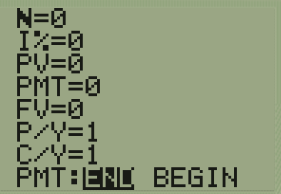
\includegraphics[width=1.8in]{TVMintro}
\end{center}

Notice the entry for PMT (on the fourth line), which we did not use last time.  This is the same as the payment amount $PMT$ in our formulas in this section.

\paragraph{Savings vs. Payout Annuities} The main difference to keep in mind when using the TVM solver is that for a savings annuity, we're using payments to build to a \emph{future value} FV, and with a payout annuity, we have a \emph{present value} PV that gets paid out in regular payments.

So for a problem involving a savings annuity, set PV to 0 and use FV and PMT (find whichever we need to based on knowing the other), and for a payout annuity, set FV to 0 and use PV and PMT.\\

The rest of the information in the menu is the same as before.  In almost every problem, if not every single one, payments occur monthly, so P/Y, and C/Y will both be 12.  Recall that I\% should be entered in percentage form, not decimal form, and you should be all set!\\

We'll show one example for each kind of annuity; both will be repeated from earlier examples for comparison.

\begin{example}[https://www.youtube.com/watch?v=m9m20XU1v-U&list=PLfmpjsIzhztsZtnb7HnXrQ8SLoiOCIcAM&index=32]{TVM Solver: Future Value for Savings Annuity}
If you deposit \$250 each month into an IRA earning 7\% interest, how much will you have in the account after 35 years?

\sol
Open the TVM solver and enter the information given (remember that N is the total number of payments, so enter \texttt{12*35}.  When you're done, you should have the following:
\begin{center}
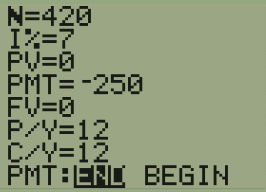
\includegraphics[width=1.8in]{TVMSavingsAnnuityFutureValue}
\end{center}
To solve for the future value, move the cursor over the value for FV, and press $\boxed{\textrm{ALPHA}}$ then $\boxed{\textrm{ENTER}}$ to solve.  You should see the answer entered there:
\begin{center}
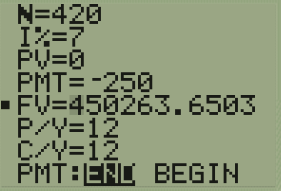
\includegraphics[width=1.8in]{TVMSavingsAnnuityFutureValueSolved}
\end{center}
The final balance will be \$450,264 (verify that this matches what we found using the formula earlier).
\end{example}

\begin{example}[https://www.youtube.com/watch?v=QF27dvKPIJ8&list=PLfmpjsIzhztsZtnb7HnXrQ8SLoiOCIcAM&index=33]{TVM Solver: Payment for Payout Annuity}
You expect to have \$500,000 in your IRA when you retire, and you want to be able to take monthly withdrawals for a total of 30 years.  If your account earns 8\% interest, how much will you be able to withdraw each month?

\sol
Here's the setup (remember, set FV to 0 and work with PV and PMT):
\begin{center}
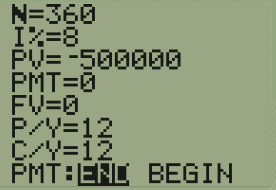
\includegraphics[width=1.8in]{TVMPayoutAnnuityPayment}
\end{center}
Remember that we use negative numbers to indicate money we spend or save, and positive for money we receive (if you forget to do this during setup, it doesn't cause any problems; just mentally reverse the signs).  After solving, you should see this:
\begin{center}
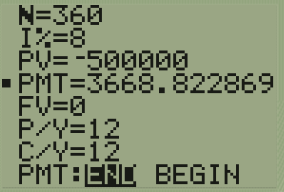
\includegraphics[width=1.8in]{TVMPayoutAnnuityPaymentSolved}
\end{center}
Notice that the answer is slightly different from the one we got using the formula (within a dollar or two), because we rounded partway through that problem.
\end{example}

\begin{try}
Try using the TVM solver to work out the other examples in this section.
\end{try}
\vfill
\pagebreak

\subsection{Using Excel}
Excel has built-in formulas to solve the same problems:
\paragraph{Finding the payment} \texttt{PMT(rate,nper,pv,[fv],[type])}
\paragraph{Finding the future value for a savings annuity} \texttt{FV(rate,nper,pmt,[pv],[type])}
\paragraph{Finding the present value for a payout annuity} \texttt{PV(rate,nper,pmt,[fv],[type])}

In each formula, the items in brackets are optional, and we won't use them here (in case you're curious, the ``type'' is the same as the option at the bottom of the TVM solver to switch between beginning-of-month and end-of-month payments).\\

\paragraph{Important note:} the rate used in these formulas is the \textbf{monthly} rate, or the given annual interest rate divide by 12.  Also, nper refers to the number of periods, which is $nt$ in our formulas.

We'll show one example here: calculating the future value of a savings annuity.

\begin{example}{Excel: Future Value for Savings Annuity}
If you deposit \$250 each month into an IRA earning 7\% interest, how much will you have in the account after 35 years?

\sol
Here's the result in Excel:
\begin{center}
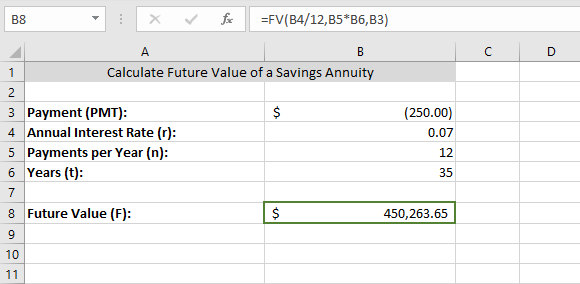
\includegraphics[width=3.5in]{ExcelSavingsAnnuityFutureValue}
\end{center}

Note that the payment amount has parentheses around it; in accounting worksheets, this is how negative values are often indicated.  The convention here is the same as with the TVM solver; since these are payments going out, we count them as negative.\\

\paragraph{Formula:} in cell B8, we entered \texttt{=FV(B4/12,B5*B6,B3)}.  Remember that the rate should be the monthly interest rate, which is why we divided the given annual rate by 12, and the value of nper is equal to the number of payments per year times the number of years.
\end{example}

\begin{try}
Try using Excel to work out the other examples in this section.
\end{try}
\vfill
\pagebreak

\subsection{Deriving the Formulas (optional)}
In case you're \emph{very} curious, and would like to see how the formulas for savings and payout annuities are derived, you can read this.  You can freely skip this part, though, without missing anything major.

\paragraph{Savings Annuity Formula}
Suppose you deposit $P$ dollars (we'll rename this $PMT$ at the end) into a savings annuity each year, and this account earns an interest rate of $r$ compounded annually (we'll handle the case of other compounding periods after we get to the formula).  At the end of the first year, the account contains $P$ dollars:
\[F_1 = P\]
This principal earns interest the second year [growing to $P(1+r)$] so at the end of the second year, the account holds that plus the newly deposited $P$:
\[F_2 = P+P(1+r)\]
Now, in the third year, this balance earns interest again: $(P+P(1+r))(1+r) = P(1+r) + P(1+r)(1+r)$, so the balance at the end of the third year is this plus another $P$:
\[F_3 = P + P(1+r) + P(1+r)^2\]
We can now see the pattern, so we can jump to the arbitrary case; at the end of $t$ years, the account will hold
\begin{equation}
F_t = P + P(1+r) + P(1+r)^2 + P(1+r)^3 + \ldots + P(1+r)^{t-1}
\end{equation}

Now comes the tricky part: we want a simpler formula for $F_t$, so we solve for it in an unexpected way.  First, multiply both sides of the last line by $(1+r)$:
\begin{equation}
F_t + F_tr = P(1+r) + P(1+r)^2 + P(1+r)^3 + \ldots + P(1+r)^{t-1} + P(1+r)^t
\end{equation}
Next, subtract equation (1.1) from equation (1.2), subtracting on both sides of the equation.  Notice that as we do so, almost all of the terms cancel:
\[F_tr = P(1+r)^t-P = P\left[(1+r)^t-1\right]\]
Finally, divide both sides of the equation by $r$ to isolate $F_t$:
\[F_t = \dfrac{P\left[(1+r)^t-1\right]}{r}\]

What if we make deposits monthly rather than yearly?  We'll assume, first of all, that the rate at which we make deposits and the rate at which interest is compounded is the same; in other words, we won't make monthly deposits to an account that compounds weekly, for instance.  If the compounding and the rate of deposit are both represented by $n$, we change this formula in the same way that we changed the compound interest formula to handle different compounding periods:
\begin{itemize}
\item Replace $r$, the annual interest rate, with $\dfrac{r}{n}$, splitting it into compounding periods.
\item Replace $t$ with $nt$ to account for the interest compounding $n$ times per year for $t$ years.
\item Rename $P$ as $PMT$ to emphasize that this is a regular payment.
\end{itemize}
This leads to the general formula:
\[\boxed{F=\dfrac{PMT\left[\left(1+\dfrac{r}{n}\right)^{nt}-1\right]}{\left(\dfrac{r}{n}\right)}}\]

\paragraph{Payout Annuity Formula}
Suppose an account holds $P$ dollars at the beginning, and this will be paid out in regular payments in the amount of $PMT$ dollars each month (or other period, determined by $n$, but this won't affect this derivation).

This account is being drained by these payments, but at the same time, interest is accruing on the remaining balance.  Thus, it turns out the future value that this account would have if it were allowed to grow by compound interest is equal to the future value it has as the reverse of a savings annuity (you can view it as the bank investing in you rather than you investing in the bank).

The future value from compound interest is \[F = P\left(1 + \dfrac{r}{n}\right)^{nt}\]
and the future value as a (reverse) savings annuity is \[F=\dfrac{PMT\left[\left(1+\dfrac{r}{n}\right)^{nt}-1\right]}{\left(\dfrac{r}{n}\right)}\]

Thus, if we set these equal to each other, we get
\[P\left(1 + \dfrac{r}{n}\right)^{nt}=\dfrac{PMT\left[\left(1+\dfrac{r}{n}\right)^{nt}-1\right]}{\left(\dfrac{r}{n}\right)}\]
and all we have to do is solve for $P$, the lump sum amount at the start of the payout process.

To do this, let's rewrite the right-hand side by separating out the denominator:
\[P\left(1 + \dfrac{r}{n}\right)^{nt}=PMT\left(\dfrac{1}{\dfrac{r}{n}}\right)\left[\left(1+\dfrac{r}{n}\right)^{nt}-1\right]\]

Now, if we divide both sides by \[\left(1 + \dfrac{r}{n}\right)^{nt}\] we only need to divide that through the last set of brackets on the right hand side:
\begin{align*}
P &= PMT\left(\dfrac{1}{\dfrac{r}{n}}\right)\dfrac{\left[\left(1+\dfrac{r}{n}\right)^{nt}-1\right]}{\left(1 + \dfrac{r}{n}\right)^{nt}}
\end{align*}

Conveniently, that is the same as the first term in brackets, so that part of the division yields 1, and the rest becomes \[\dfrac{1}{\left(1 + \dfrac{r}{n}\right)^{nt}}.\]
Recall that we can use negative exponents to move terms from the denominator to the numerator, so
\[\dfrac{\left[\left(1+\dfrac{r}{n}\right)^{nt}-1\right]}{\left(1 + \dfrac{r}{n}\right)^{nt}} = \left[1-\left(1 + \dfrac{r}{n}\right)^{-nt}\right]\]

Putting the pieces back together gives the final formula:
\[\boxed{P = \dfrac{PMT\left[1-\left(1+\dfrac{r}{n}\right)^{-nt}\right]}{\left(\dfrac{r}{n}\right)}}\]